\documentclass{thesis_proposal}

\title{Improving web accessibility by integrating continuous evaluation to development workflow}
\author{Mariann Tapfer}
\email{tapferm@gmail.com}

\begin{document}
\maketitle

% TODO format abstract and keywords/supervisors better
\begin{abstract}
    Improving accessibility is often a struggle, but understanding the extent of the problem and keeping a close eye on it throughout the lifespan of the product could make it more manageable. Continuous integration helps improve and maintain code quality. Could integrating automated accessibility evaluation to the CI pipeline improve the accessibility of the end product in a similar way?
\end{abstract}
\keywords{Web Accessibility, Automatic Evaluation, Continuous Integration, CRM software}
\supervisor{David Jose Ribera Lamas, Mustafa Can Özdemir, Mari-Ell Mets}

\section{Problem Statement}
According to WHO 1 billion people or about 15\% of the world's population are estimated to experience disability \citep{WHO_disability_2021}. They need web accessible web applications. There is proof that focusing on accessibility has a profound effect on overall quality of products and services and therefore provides a big business value \citep{miesenberger_user_2020}.
Developers find it hard to maintain a high level of accessibility over time as it is considered more at the first release of the product \citep{paterno_requirements_2020}. Continuous integration is used to speed up development and maintain general code quality \citep{zhao_impact_2017} and it could also help in maintaining a high level of accessibility by testing the added code against predefined accessibility requirements. There is some initial research into the current state of accessibility testing in continuous integration, but it could be improved by doing a case study for an organisation \citep{sane_brief_2021}.


\section{Research Goal and Research Questions}
This thesis will first map the different automated accessibility evaluation tools to understand their pros and cons and then test out one of them in a web based CRM development process to determine if this practice could help developers make a more accessible product. CRM software was chosen because usability for users with varied abilities is an important aspect in a CRM software indicated by ease of use and learnability often being mentioned in their reviews \citep{sevilla_best_2022, 23_best_CRM}.

\begin{RQlist}
    \item What kind of errors can automated accessibility testing catch?
    \item Can integrating automated testing to a web based CRM’s development pipeline help improve the compliance of the end products with WCAG standards?
    \item Can integrating automated testing to the development pipeline help improve developers’ awareness and knowledge about accessibility standards?
    \item What are the biggest problems in integrating automated accessibility testing software to development workflow?
\end{RQlist}

\section{Methods}
A literature review will be conducted to map current practices in automating accessibility evaluation. Focusing on more recent articles and software that would be compatible with the company later used in the case study.
User centred research approach will be used, where developers are users, in order to find out what effect could integration of an automated accessibility testing have on the end product and the participants knowledge on the subject.
Some initial testing will be conducted to prepare examples of what kind of automated testing could be used to detect accessibility problems. The developers from the front-end platform team will decide what kind of approach would be most beneficial and what library or service should be tested.
After the selection test set up will be configured and some initial test and documentation on how to understand the results and make changes will be added.
All the developers involved will be asked to fill out a pre and post test questionnaire to determine their level of knowledge and attitude prior to the intervention and see if these improve. Not all developers will work on the same service or library equally during the research period and some might not even come into contact with it. Developers with most experience with the tests during the intervention will be chosen to carry out interviews to understand their experience better.

\section{Research Plan}
Initial research about automated accessibility evaluation tools will be carried out in order to understand the problems and possibilities of this approach and to gain necessary background knowledge to be able to understand and analyse the results of the intervention.
The case study should be started as soon as possible in order to see its potential impact over time and other activities are planned around it (see figure~\ref{fig:plan}).
In addition to publications in academic journals, articles from the most influential web pages and blogs in the field should be included to get the most up to date information.
\begin{figure}[ht!]
	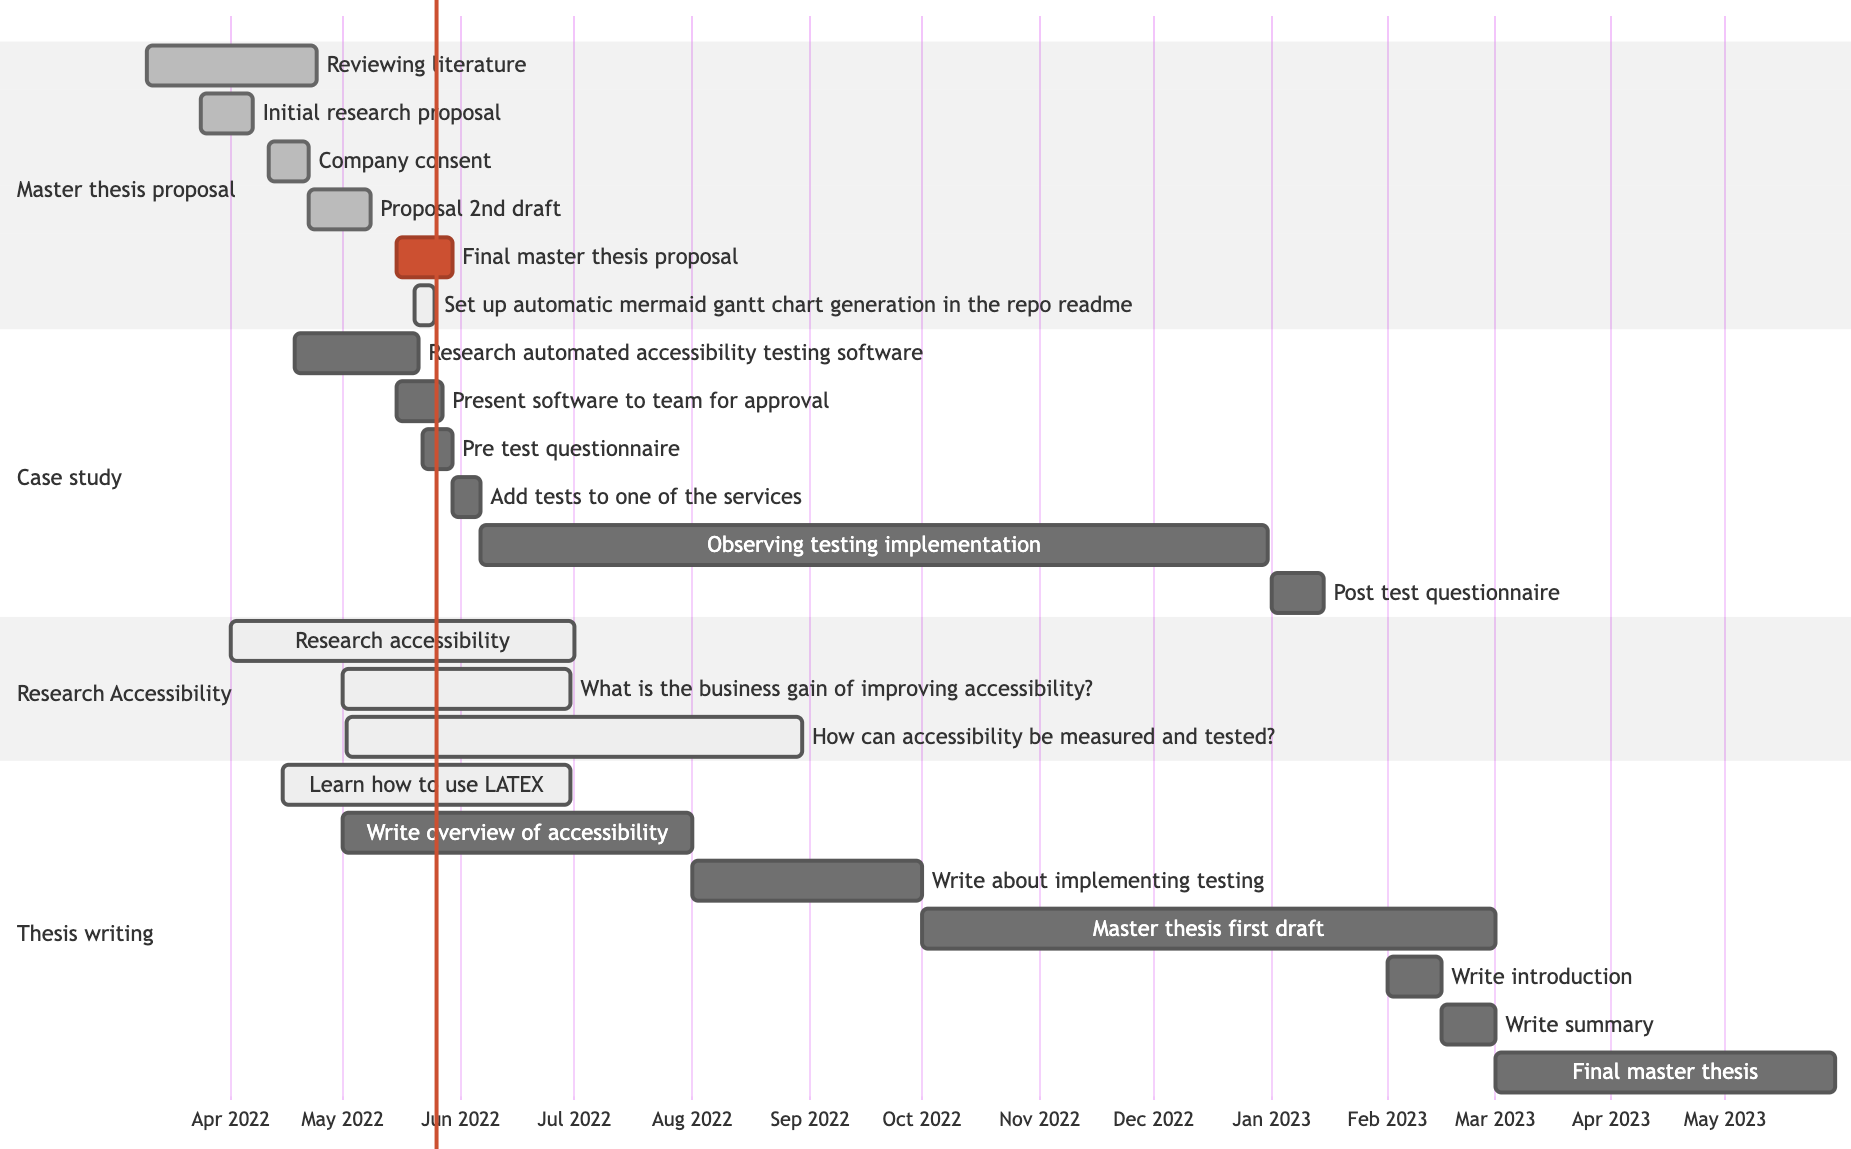
\includegraphics[width=1\textwidth]{img/timeline.png}
	\caption{Master thesis work plan}\label{fig:plan}
\end{figure}

\pagebreak
\printbibliography{}
\nocite{*}

\end{document}